% Created by tikzDevice version 0.10.1 on 2017-10-23 14:01:54
% !TEX encoding = UTF-8 Unicode
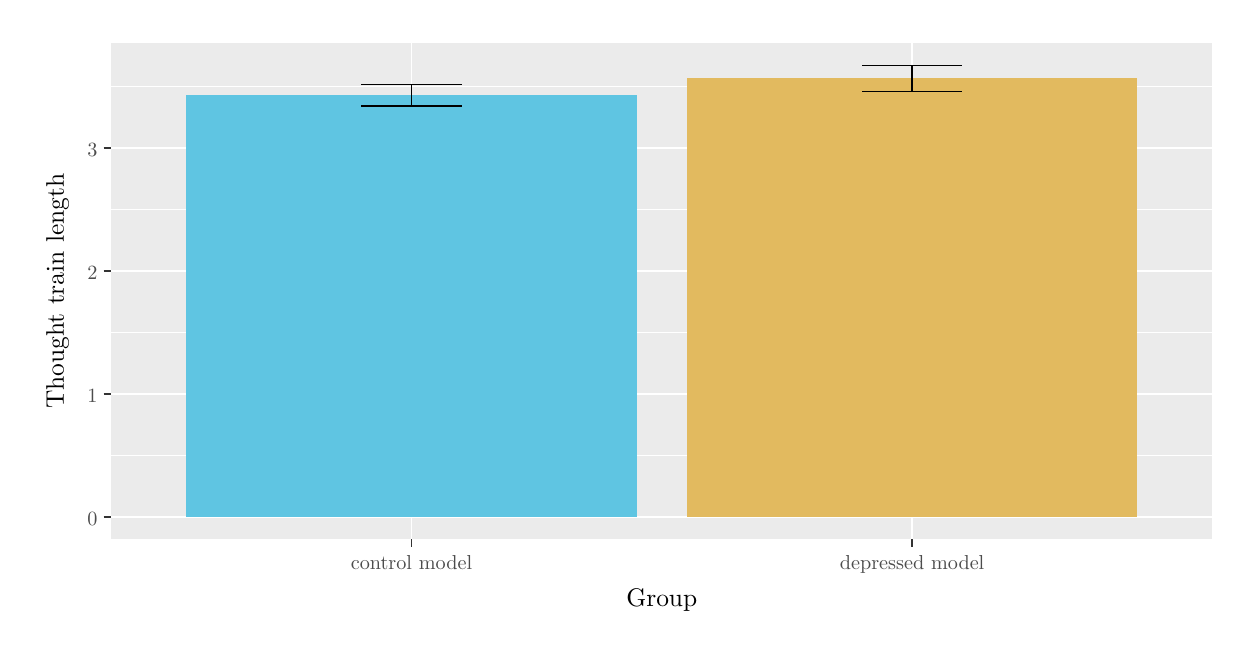
\begin{tikzpicture}[x=1pt,y=1pt]
\definecolor{fillColor}{RGB}{255,255,255}
\path[use as bounding box,fill=fillColor,fill opacity=0.00] (0,0) rectangle (433.62,216.81);
\begin{scope}
\path[clip] (  0.00,  0.00) rectangle (433.62,216.81);
\definecolor{drawColor}{RGB}{255,255,255}
\definecolor{fillColor}{RGB}{255,255,255}

\path[draw=drawColor,line width= 0.6pt,line join=round,line cap=round,fill=fillColor] (  0.00,  0.00) rectangle (433.62,216.81);
\end{scope}
\begin{scope}
\path[clip] ( 30.17, 31.92) rectangle (428.12,211.31);
\definecolor{fillColor}{gray}{0.92}

\path[fill=fillColor] ( 30.17, 31.92) rectangle (428.12,211.31);
\definecolor{drawColor}{RGB}{255,255,255}

\path[draw=drawColor,line width= 0.3pt,line join=round] ( 30.17, 62.28) --
	(428.12, 62.28);

\path[draw=drawColor,line width= 0.3pt,line join=round] ( 30.17,106.68) --
	(428.12,106.68);

\path[draw=drawColor,line width= 0.3pt,line join=round] ( 30.17,151.09) --
	(428.12,151.09);

\path[draw=drawColor,line width= 0.3pt,line join=round] ( 30.17,195.49) --
	(428.12,195.49);

\path[draw=drawColor,line width= 0.6pt,line join=round] ( 30.17, 40.07) --
	(428.12, 40.07);

\path[draw=drawColor,line width= 0.6pt,line join=round] ( 30.17, 84.48) --
	(428.12, 84.48);

\path[draw=drawColor,line width= 0.6pt,line join=round] ( 30.17,128.88) --
	(428.12,128.88);

\path[draw=drawColor,line width= 0.6pt,line join=round] ( 30.17,173.29) --
	(428.12,173.29);

\path[draw=drawColor,line width= 0.6pt,line join=round] (138.70, 31.92) --
	(138.70,211.31);

\path[draw=drawColor,line width= 0.6pt,line join=round] (319.59, 31.92) --
	(319.59,211.31);
\definecolor{fillColor}{RGB}{95,197,226}

\path[fill=fillColor] ( 57.30, 40.07) rectangle (220.10,192.37);
\definecolor{fillColor}{RGB}{226,186,95}

\path[fill=fillColor] (238.19, 40.07) rectangle (400.99,198.47);
\definecolor{drawColor}{RGB}{0,0,0}

\path[draw=drawColor,line width= 0.6pt,line join=round] (120.61,196.28) --
	(156.79,196.28);

\path[draw=drawColor,line width= 0.6pt,line join=round] (138.70,196.28) --
	(138.70,188.46);

\path[draw=drawColor,line width= 0.6pt,line join=round] (120.61,188.46) --
	(156.79,188.46);

\path[draw=drawColor,line width= 0.6pt,line join=round] (301.50,203.16) --
	(337.68,203.16);

\path[draw=drawColor,line width= 0.6pt,line join=round] (319.59,203.16) --
	(319.59,193.78);

\path[draw=drawColor,line width= 0.6pt,line join=round] (301.50,193.78) --
	(337.68,193.78);
\end{scope}
\begin{scope}
\path[clip] (  0.00,  0.00) rectangle (433.62,216.81);
\definecolor{drawColor}{gray}{0.30}

\node[text=drawColor,anchor=base east,inner sep=0pt, outer sep=0pt, scale=  0.73] at ( 25.22, 37.04) {0};

\node[text=drawColor,anchor=base east,inner sep=0pt, outer sep=0pt, scale=  0.73] at ( 25.22, 81.45) {1};

\node[text=drawColor,anchor=base east,inner sep=0pt, outer sep=0pt, scale=  0.73] at ( 25.22,125.85) {2};

\node[text=drawColor,anchor=base east,inner sep=0pt, outer sep=0pt, scale=  0.73] at ( 25.22,170.26) {3};
\end{scope}
\begin{scope}
\path[clip] (  0.00,  0.00) rectangle (433.62,216.81);
\definecolor{drawColor}{gray}{0.20}

\path[draw=drawColor,line width= 0.6pt,line join=round] ( 27.42, 40.07) --
	( 30.17, 40.07);

\path[draw=drawColor,line width= 0.6pt,line join=round] ( 27.42, 84.48) --
	( 30.17, 84.48);

\path[draw=drawColor,line width= 0.6pt,line join=round] ( 27.42,128.88) --
	( 30.17,128.88);

\path[draw=drawColor,line width= 0.6pt,line join=round] ( 27.42,173.29) --
	( 30.17,173.29);
\end{scope}
\begin{scope}
\path[clip] (  0.00,  0.00) rectangle (433.62,216.81);
\definecolor{drawColor}{gray}{0.20}

\path[draw=drawColor,line width= 0.6pt,line join=round] (138.70, 29.17) --
	(138.70, 31.92);

\path[draw=drawColor,line width= 0.6pt,line join=round] (319.59, 29.17) --
	(319.59, 31.92);
\end{scope}
\begin{scope}
\path[clip] (  0.00,  0.00) rectangle (433.62,216.81);
\definecolor{drawColor}{gray}{0.30}

\node[text=drawColor,anchor=base,inner sep=0pt, outer sep=0pt, scale=  0.73] at (138.70, 20.91) {control model};

\node[text=drawColor,anchor=base,inner sep=0pt, outer sep=0pt, scale=  0.73] at (319.59, 20.91) {depressed model};
\end{scope}
\begin{scope}
\path[clip] (  0.00,  0.00) rectangle (433.62,216.81);
\definecolor{drawColor}{RGB}{0,0,0}

\node[text=drawColor,anchor=base,inner sep=0pt, outer sep=0pt, scale=  0.92] at (229.14,  7.83) {Group};
\end{scope}
\begin{scope}
\path[clip] (  0.00,  0.00) rectangle (433.62,216.81);
\definecolor{drawColor}{RGB}{0,0,0}

\node[text=drawColor,rotate= 90.00,anchor=base,inner sep=0pt, outer sep=0pt, scale=  0.92] at ( 13.08,121.61) {Thought train length};
\end{scope}
\end{tikzpicture}
